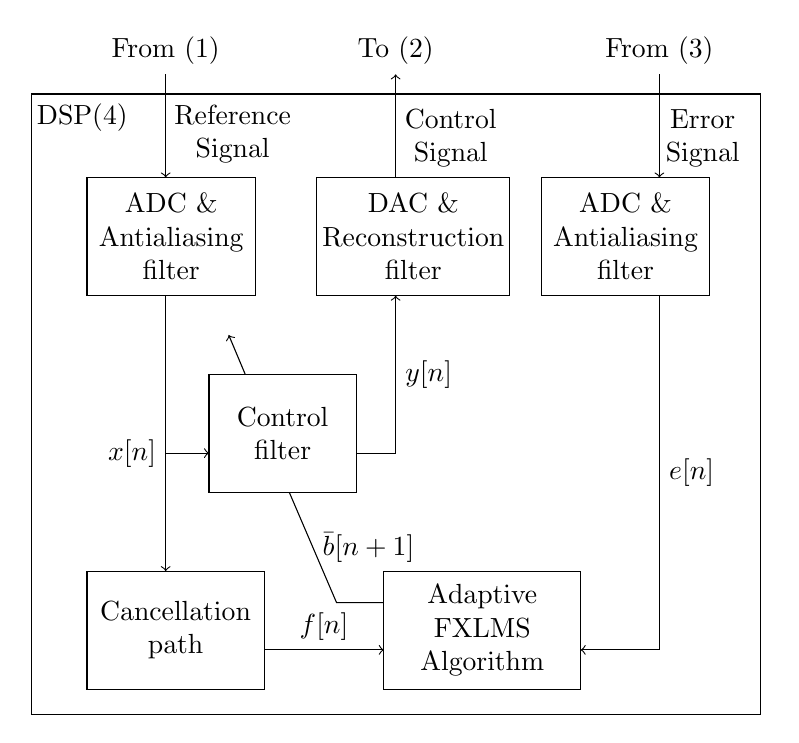
\begin{tikzpicture}

\draw  (-3,5) rectangle node[text width=2cm,align=center] {ADC \& Antialiasing filter} (-0.86,3.5);
\draw  (-3,0) rectangle node[text width=2.5cm,align=center] {Cancellation path}(-0.75,-1.5);
\draw  (0.77,0) rectangle node[text width=2.5cm,align=center] {Adaptive FXLMS Algorithm} (3.27,-1.5);

\draw  (-1.45,2.5) rectangle node[text width=1.5cm,align=center,fill=white] {Control filter} (0.42,1);
\draw  (-0.08,5) rectangle node[text width=2.5cm,align=center] {DAC \& \\ Reconstruction filter}(2.37,3.5);
\draw  (2.77,5) rectangle node[text width=2cm,align=center] {ADC \& Antialiasing filter}(4.91,3.5);

\draw  (-3.71,6.06) rectangle (5.55,-1.82);
\node at (-3.06,5.76) {DSP(4)};
\node [text width=2cm,align=center] at (-1.15,5.55) {Reference Signal};

\draw[->] (-0.75,-1) -- node[above]{$f[n]$} (0.77,-1);

\draw[->] (4.27,3.5) -- node[right]{$e[n]$} (4.27,-1)  -- (3.27,-1);

\draw [->](4.27,6.31) node[above]{From (3)} -- (4.27,5) ;
\draw [->](0.92,5)  --  (0.92,6.31) node[above]{To (2)};
\draw [->](-2,3.5) -- (-2,0);

\draw [->](-2,1.5) node[left]{$x[n]$} -- (-1.45,1.5);

\draw[->] (0.42,1.5) -- (0.92,1.5) --node[right]{$y[n]$} (0.92,3.5);
\draw [->](-2,6.31) node[above]{From (1)} -- (-2,5);
\node [text width=2cm,align=center] at (1.62,5.5) {Control Signal};
\node [text width=1.5cm,align=center] at (4.82,5.5) {Error Signal};

\draw (0.77,-0.4) -- (0.17,-0.4) --node[right]{$\bar{b}[n+1]$} (-0.43,1);
\draw [->](-0.99,2.5) -- (-1.2,3);
\end{tikzpicture}